\documentclass[11pt,a4paper]{article}
\usepackage[T1]{fontenc}
\usepackage[utf8]{inputenc}
\usepackage[english]{babel}
\usepackage{mathptmx,microtype}
\usepackage[margin=2.5cm]{geometry}
\usepackage{amsmath,amssymb}
\usepackage{graphicx,booktabs,caption,array}
\usepackage[hidelinks]{hyperref}
\captionsetup{font=small,labelfont=bf}
\graphicspath{{figure/}}
\setlength{\parskip}{0.35em}
\title{Volatility Risk Premium and Non-Directional Option Strategies\\ on the S\&P 500 Index:\\ Evidence from 2010--2023 SPX Option Chains\thanks{Authors: Giordano Margotti, Alex Crescentini, Alessandro Celani, Giulio Sciacchitano (\emph{finance-thinking} working group, repository \texttt{options\_strategy}). All analyses in this document were recomputed from the option chains; errors and omissions are the authors' own. This document is for research purposes and is not investment advice.}}
\author{}
\date{November 2026}
\begin{document}
{\let\newpage\relax\maketitle}
\vspace{-3em}

\begin{abstract}
\noindent This paper tests, on daily chains of European options on the S\&P 500 index from 2010 to 2023 (3,499 sessions, 47,699 date--expiry pairs), whether a volatility risk premium exists and whether non-directional option-selling strategies capture it net of costs. The answer depends on the measure. The 30-day model-free implied volatility exceeds subsequently realized volatility by +3.45 points on average ($t$-statistic 6.48), whereas at-the-money implied volatility exceeds it by only +0.72 points ($t$ 1.36): the premium sits in the wings of the distribution, in out-of-the-money puts in particular, not in the central level of the surface. The at-the-money premium is significant in 2010--2014 and statistically zero in the two following sub-periods. Across 434 configurations of ten strategy families (1,310,509 simulated trades), the median Sharpe ratio is +0.39 at mid prices and $-$0.40 at bid-ask prices; the share of configurations with a significantly positive alpha against the index falls from 16.4\% to 2.5\%. Positive results are concentrated in structures that sell puts and are largely explained by equity market exposure. The evidence is consistent with a premium that exists as compensation for tail risk, but that the bid-ask spread and ex-post parameter selection make hard to capture systematically.

\medskip\noindent\textbf{Keywords:} volatility risk premium, implied volatility, index options, iron condor, put credit spread, GJR-GARCH, transaction costs, multiple testing.
\end{abstract}

\section{Introduction}

The project behind this document explores the possibility of generating excess returns through non-directional option strategies, that is, strategies whose result does not depend on the direction of the underlying as long as the price stays within a range or volatility remains contained. These are premium-selling strategies: iron condors, strangles, put credit spreads and related structures. The project's framing document identifies three sources of expected return: range-bound behavior of the price, the time decay of option value, and the existence of a volatility risk premium (VRP), namely a systematic difference between the volatility implied by option prices and the volatility the underlying subsequently realizes.

The first two are not expected returns in a strict sense. Time decay is the price of exposure to convexity: in a market where options are fairly priced, the theta collected offsets gamma losses on average. Range-bound behavior is already embedded in the premium. The only source of positive expected return for an option seller is therefore the third: an option price above the expected value of its payoff under the real-world measure. The research question is accordingly twofold:
\begin{enumerate}
\item whether the volatility risk premium exists in the data, how large it is, in which region of the volatility surface it lies and how stable it is over time;
\item whether the non-directional strategies examined by the project capture it, once the bid-ask spread, commissions, margin and the number of configurations tried are taken into account.
\end{enumerate}

The contribution is empirical. All statistics are computed on end-of-day quotes of SPX options from January 4, 2010 to December 29, 2023, with a deliberately simple and reproducible design: implied volatility obtained from prices with the Black (1976) model on the forward implied by put-call parity, model-free implied variance with the Cboe formula, realized variance up to the expiry of the same option, and a GJR-GARCH(1,1) forecast with Student-$t$ innovations estimated on an expanding window with no look-ahead. Code and results are published in the repository together with an interactive site for exploring every configuration.

The document is organized as follows. Section~\ref{sec:lett} summarizes the literature on the existence, causes and persistence of the premium. Section~\ref{sec:dati} describes data and method. Section~\ref{sec:vrp} presents the evidence on the premium; Section~\ref{sec:strat} the strategy backtests; Section~\ref{sec:rob} the robustness checks and the multiple-testing correction. Section~\ref{sec:codice} documents the checks on the pre-existing code. Sections~\ref{sec:limiti} and~\ref{sec:concl} discuss limitations and conclusions.

\section{Literature}\label{sec:lett}

\subsection{Definition and evidence}

The variance risk premium is the difference between the expected future variance under the risk-neutral measure and its expectation under the real-world measure. The first term is observable: Britten-Jones and Neuberger (2000) show that risk-neutral expected variance can be replicated with a static portfolio of options across all strikes, with no model assumption; Jiang and Tian (2005) study its information content, and the VIX index is its market implementation. Carr and Wu (2009) build synthetic variance swap rates for indices and individual stocks and document that, for US equity indices, implied variance systematically exceeds realized variance: variance sellers earn a large and statistically significant average premium. Bakshi and Kapadia (2003) reach the same conclusion with a different strategy, showing that the gain of a purchased, delta-hedged option is negative on average. Coval and Shumway (2001) find strongly negative average returns for zero-delta straddles, and Bondarenko (2014) quantifies the historical cost of index puts: average monthly losses of several tens of percent for out-of-the-money puts. Bollerslev, Tauchen and Zhou (2009) further show that the difference between implied and realized variance predicts equity returns at the quarterly horizon, which qualifies it as a measure of the price of risk rather than a mere forecast error.

\subsection{Why the premium would exist}

The proposed explanations fall into three groups.

\emph{Compensation for systematic risk.} Variance rises when markets fall; a security that pays in those states has insurance value and its seller must be compensated. Bates (2000) documents that, after the 1987 crash, option prices persistently embed the fear of negative jumps. Todorov (2010) and Bollerslev and Todorov (2011) attribute the larger part of the premium to compensation for jump risk, that is, to the tails, rather than to diffusive volatility. Dew-Becker, Giglio, Le and Rodriguez (2017) show that the price of risk is concentrated on very short-term realized variance, while news about future variance is priced close to zero.

\emph{Hedging demand and intermediary constraints.} Bollen and Whaley (2004) link the shape of the volatility smile to the net buying pressure on index puts. Gârleanu, Pedersen and Poteshman (2009) build a model in which intermediaries cannot hedge perfectly and end-user demand moves option prices in proportion to the unhedgeable risk. In this framework the premium is the compensation of those who provide balance-sheet capacity, and it varies with it.

\emph{Preferences and perceptions.} Jackwerth (2000) recovers from options an implied risk aversion that is incompatible with standard preferences after 1987; Ilmanen (2012) summarizes the evidence that, across asset classes, selling insurance against tails has been rewarded and buying lottery-like exposures has been penalized.

\subsection{The efficiency view}

A positive average premium does not contradict market efficiency in the sense of Fama (1970): a positive expected return for bearing systematic risk is an equilibrium price, not an anomaly. The relevant question is whether the premium exceeds the compensation justified by the risk and whether it can be captured.

On both points the literature offers reasons for caution. Broadie, Chernov and Johannes (2009) show that very negative average put returns are not, by themselves, evidence of mispricing: standard models with stochastic volatility and jumps generate returns of that order, and available samples are too short to distinguish a high premium from the absence, in the sample, of the rare events that justify it. Santa-Clara and Saretto (2009) show that margin requirements and transaction costs drastically reduce the returns actually obtainable from selling options: an investor must hold substantial cash to survive margin calls, and the implementable strategy is a fraction of the theoretical one. Constantinides, Jackwerth and Savov (2013) document that the usual risk factors do not explain index option returns without adding specific jump and volatility factors. Jurek and Stafford (2015) show that the return profile of many alternative funds can be replicated by selling index puts and that, valued at the cost of capital appropriate for that tail risk, the apparent alpha disappears. Israelov and Nielsen (2015) decompose the return of covered-call strategies into equity exposure, short volatility exposure and unintended timing, and show that most of the return is equity beta.

On the forecasting side, more recent work has rehabilitated implied volatility. Canina and Figlewski (1993) found no information content; Christensen and Prabhala (1998), with non-overlapping samples, show that implied volatility is a nearly unbiased and efficient forecast of realized volatility; the survey by Poon and Granger (2003) confirms that implied volatility generally outperforms time-series models.

Finally, the premium is not constant. Dew-Becker and Giglio (2023, 2025) document that over the last fifteen years index option alphas have become statistically indistinguishable from zero and that the variance risk premium has shrunk, consistent with a model in which option prices are determined by intermediaries and the cost of hedging has declined. For same-day expiries, Beckmeyer, Branger and Gayda (2023) estimate that retail investors lost in aggregate on zero-days-to-expiry SPX options, largely because of trading costs.

\subsection{Implications for the project}

Four predictions that can be tested on the available data follow from the literature: (i) the premium measured with model-free variance must be larger than the one measured on at-the-money volatility, because the larger part is compensation for the tails; (ii) the distribution of the realized premium must be strongly left-skewed; (iii) the premium must be weaker in the recent part of the sample; (iv) the returns of selling strategies must shrink markedly once costs and equity market exposure are considered. The following sections test them one by one.

\section{Data and method}\label{sec:dati}

\subsection{Data}

The source is OptionsDX (\url{https://www.optionsdx.com}), dataset \emph{SPX Option Chains} at end-of-day frequency: monthly files \texttt{spx\_eod\_YYYYMM} from January 2010 to December 2023, obtained through the working group's repository. Each file contains the full option chain of every session at the close, with one row per expiry--strike pair and, for each side, bid, ask, volume, the vendor's implied volatility and Greeks, together with the level of the underlying.

The instrument is the option on the S\&P 500 index listed on the Cboe Options Exchange (ticker SPX): a European-style, cash-settled index option with a multiplier of 100 dollars per index point. The archive includes the standard third-Friday monthly expiries, settled on the opening value, and the weekly and end-of-month expiries (SPXW), settled on the closing value. The archive contains 3,499 sessions; the only gap longer than five calendar days falls in January 2011. The analyses use expiries with 1 to 75 calendar days to expiry. The index level is the one reported in the chains at the close.

Dollar results refer to one SPX contract; for the XSP contract, one tenth the size, values are divided by ten, while per-contract commissions are unchanged and therefore weigh ten times more in relative terms.

\subsection{Forward, implied volatility and delta}

For each date--expiry pair the implied forward $F$ is obtained from put-call parity at the strike where call and put mid prices are closest: $F = K^\ast + C(K^\ast) - P(K^\ast)$. Dividends and rates thus enter through the market and require no external assumption; the discount factor on the premium, negligible at the maturities considered, is set to one. The implied volatility of each option is obtained by bisection on the Black (1976) formula applied to the mid price, with $T$ equal to calendar days divided by 365; delta is the forward delta of the same model. At-the-money volatility is the linear interpolation in strike, at $K=F$, of the volatilities of out-of-the-money options.

The integrity checks give the expected results: the inversion reproduces prices with a maximum error of the order of $10^{-5}$ index points; at $K=F$ the implied volatilities of put and call coincide (zero median difference, 5th and 95th percentiles within a tenth of a volatility point); call delta minus put delta equals one; the cost of carry implied by the forward is consistent with the level of rates net of dividends year by year.

\subsection{Model-free implied variance}

Model-free implied variance follows the VIX formula applied to the single expiry:
\begin{equation}
\sigma^2_{\mathrm{MF}} = \frac{2}{T}\sum_i \frac{\Delta K_i}{K_i^2}\, Q(K_i) - \frac{1}{T}\left(\frac{F}{K_0}-1\right)^2 ,
\end{equation}
where $Q(K_i)$ is the mid price of the out-of-the-money option with strike $K_i$, $K_0$ is the first strike not above $F$ and the sum stops, on each side, after two consecutive zero bids. The mean of $\sigma_{\mathrm{MF}}$ on the expiry closest to 30 days is 18.06\%, in line with the order of magnitude of the VIX index over the period.

\subsection{Realized variance and definition of the premium}

For an option observed at $t$ with expiry at $t+T$, realized variance is the sum of squared daily log returns from the session after $t$ to expiry, divided by $T$ in calendar years:
\begin{equation}
RV_{t,T} = \frac{1}{T}\sum_{s=t+1}^{t+T} r_s^2 .
\end{equation}
Implied and realized are thus annualized over the same calendar interval and refer to exactly the same period. The premium is reported in three forms: in volatility points on the at-the-money measure, $\sigma_{\mathrm{ATM}} - \sqrt{RV}$; in volatility points on the model-free measure, $\sigma_{\mathrm{MF}} - \sqrt{RV}$; in variance units, $\sigma^2_{\mathrm{MF}} - RV$, which corresponds to the payoff of a short variance swap.

For each target horizon (7, 14, 21, 30, 45 and 60 days) the expiry with time to expiry closest to the target, within a preset tolerance, is selected in every session. Since daily observations overlap, standard errors are Newey and West (1987) with a number of lags equal to one and a half times the horizon in sessions; statistics on the non-overlapping sample are reported as a check.

\subsection{GJR-GARCH forecast}

The reference model for expected volatility under the real-world measure is the GJR-GARCH(1,1) of Glosten, Jagannathan and Runkle (1993) with Student-$t$ innovations, an asymmetric generalization of the models of Engle (1982) and Bollerslev (1986):
\begin{equation}
\sigma^2_{t+1} = \omega + \left(\alpha + \gamma\,\mathbf{1}_{\{\varepsilon_t<0\}}\right)\varepsilon_t^2 + \beta\,\sigma_t^2 .
\end{equation}
Estimation uses an expanding window of at least 504 sessions and is repeated every 21 sessions; between estimations the conditional variance is updated with the current parameters and only with returns already observed. The forecast of total variance to expiry is the sum of daily forecasts over the $n$ remaining sessions, $\sum_{k=1}^{n}\left[\bar\sigma^2 + p^{\,k-1}(\sigma^2_{t+1}-\bar\sigma^2)\right]$, with persistence $p=\alpha+\gamma/2+\beta$ and long-run variance $\bar\sigma^2=\omega/(1-p)$, annualized over the same calendar time as the implied measure. No correction factor is applied. Forecasts are available from January 2012. In the estimated parameters $\alpha$ is zero and $\gamma$ lies between 0.24 and 0.36: in the sample, variance reacts only to negative returns.

\subsection{Backtest design}

In every session and for each target expiry (7, 14, 30 and 45 days) a unit position is opened for each configuration. Strikes are chosen by delta (0.10, 0.16, 0.20 and 0.30 for short legs); the wings of defined-risk structures follow two alternative rules: delta 0.05, or a distance equal to 1\% of spot. There are ten families: short put, short strangle, short at-the-money straddle, put credit spread, call credit spread, iron condor, iron butterfly, long put, debit put spread and long at-the-money calendar. For credit structures three management rules are considered: hold to expiry; close when profit reaches 50\% of the credit; close at 50\% profit or at a loss equal to 200\% of the credit. Exit conditions are evaluated on daily closing mid prices. In total there are 434 configurations and 1,310,509 simulated trades.

\emph{Execution prices.} For each trade the result at mid prices and the sum of the half bid-ask spreads of the legs traded, at entry and at any early exit, are recorded. The result is therefore a linear function of the share $x$ of the spread paid: $x=0$ corresponds to mid prices, $x=1$ to selling at the bid and buying at the ask. At expiry, settlement is in cash and involves no spread. The commission is one dollar per leg per contract.

\emph{Margin and return.} For defined-risk structures the margin is the maximum loss; for naked positions it is 20\% of notional, as in the group's code; for debit structures it is the premium paid. The return of each trade is the result divided by the margin. To obtain a monthly series comparable across maturities a constant-capital ladder is assumed: capital is split equally among positions open at the same time, so that each trade contributes to the return of its closing month by its return on margin divided by the number of sessions in the horizon. Monthly series are summed without compounding; mean return and maximum drawdown therefore scale linearly with the share of capital committed to margin, while the Sharpe ratio does not depend on it.

\emph{Market exposure.} For each configuration the monthly returns are regressed on the monthly returns of the index; the annualized intercept (alpha) measures the return not explained by equity exposure.

\section{The volatility risk premium in the data}\label{sec:vrp}

\subsection{Average level by horizon}

Table~\ref{tab:oriz} reports, for each horizon, the mean of at-the-money implied volatility, model-free volatility and realized volatility, with the two measures of the premium.

\begin{table}[ht]\centering\small
\caption{Implied and realized volatility by horizon, SPX 2010--2023. Values in percentage points of annualized volatility; $t$ with Newey-West standard errors.}\label{tab:oriz}
\begin{tabular}{rrrrrrrrrrrr}\toprule
 & & \multicolumn{3}{c}{Means} & \multicolumn{3}{c}{ATM $-$ realized} & \multicolumn{2}{c}{MF $-$ realized} & & \\ \cmidrule(lr){3-5}\cmidrule(lr){6-8}\cmidrule(lr){9-10}
Days & Sessions & ATM & MF & Real. & Mean & $t$ & \% $>0$ & Mean & $t$ & Skew & Min. \\ \midrule
7 & 2,892 & 15.18 & 17.09 & 13.84 & +1.34 & 5.43 & 68 & +3.25 & 13.33 & $-$3.7 & $-$99 \\
14 & 3,018 & 14.98 & 17.25 & 14.10 & +0.88 & 2.48 & 69 & +3.15 & 8.98 & $-$4.9 & $-$90 \\
21 & 3,098 & 15.09 & 17.57 & 14.33 & +0.76 & 1.72 & 68 & +3.24 & 7.31 & $-$4.9 & $-$79 \\
30 & 3,134 & 15.32 & 18.06 & 14.60 & +0.72 & 1.36 & 69 & +3.45 & 6.48 & $-$5.0 & $-$77 \\
45 & 3,104 & 15.99 & 19.06 & 15.18 & +0.81 & 1.22 & 70 & +3.88 & 5.71 & $-$4.5 & $-$71 \\
60 & 3,250 & 16.30 & 19.57 & 15.34 & +0.96 & 1.27 & 73 & +4.23 & 5.50 & $-$4.1 & $-$64 \\
\bottomrule\end{tabular}\end{table}

Three facts emerge. First, model-free volatility exceeds realized volatility by more than three points at all horizons, with $t$-statistics between 5.50 and 13.33. Second, at-the-money volatility exceeds realized volatility by less than one point beyond 14 days, and the difference is not statistically different from zero at 21, 30, 45 and 60 days; the at-the-money premium is significant only at 7 days (+1.34 points, $t$ 5.43) and at 14 days (+0.88 points, $t$ 2.48). Third, the distribution is strongly skewed. At 30 days the median at-the-money premium is +1.74 points and the premium is positive in 69.1\% of sessions, but skewness is $-$5.0 and the minimum, in February 2020, is $-$77.5 points. The mean is the sum of many small gains and a few very large losses (Figure~\ref{fig:serie}).

\begin{figure}[ht]\centering
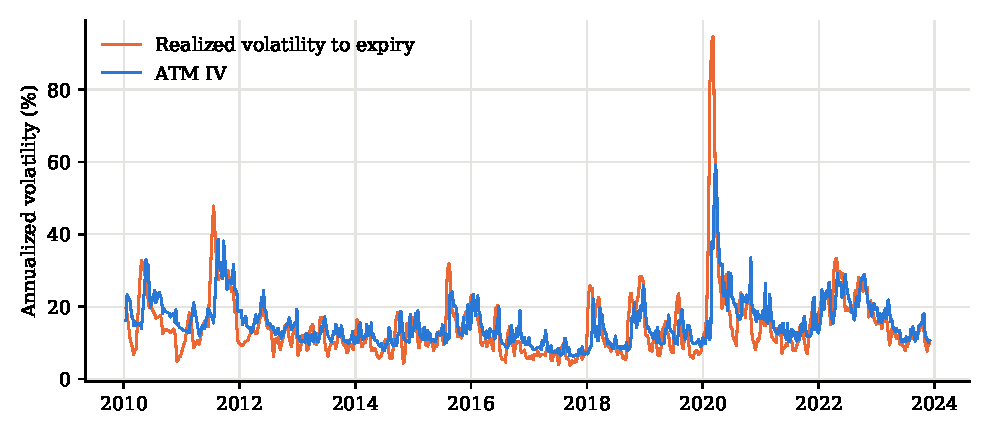
\includegraphics[width=\textwidth]{serie_en.pdf}
\caption{At-the-money implied volatility on the expiry closest to 30 days and realized volatility to that expiry. Weekly sampling.}\label{fig:serie}
\end{figure}

The distance between the two implied measures, about 2.7 points at 30 days, is the contribution of the wings. In the sample the implied volatility of the 0.10-delta put exceeds at-the-money volatility by 7.34 points on average and the difference between 0.25-delta put and call is 5.48 points. The first prediction of the literature is therefore confirmed: the premium is not in the central level of the surface, it is in the skew.

\begin{figure}[ht]\centering
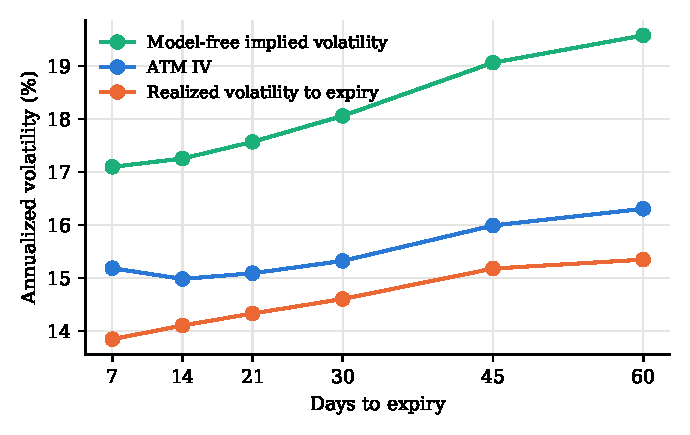
\includegraphics[width=0.48\textwidth]{struttura_en.pdf}\hfill
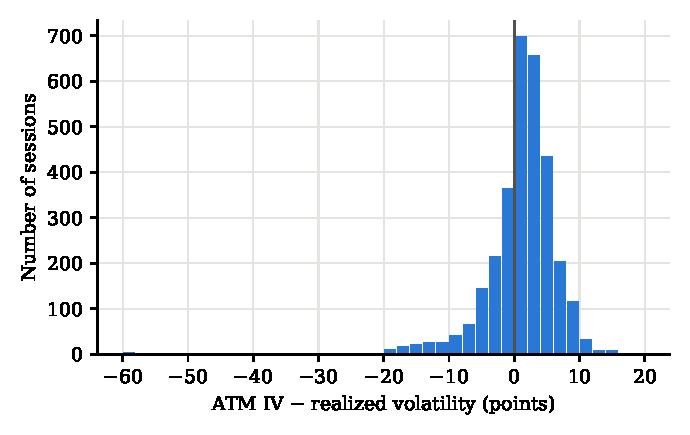
\includegraphics[width=0.48\textwidth]{isto_en.pdf}
\caption{Left: means by horizon of the three volatility measures. Right: distribution of the 30-day at-the-money premium.}\label{fig:strut}
\end{figure}

\subsection{Stability over time}

The 30-day at-the-money premium averages +1.82 points in 2010--2014 ($t$ 4.02), +0.46 points in 2015--2019 ($t$ 0.84) and +0.04 points in 2020--2023 ($t$ 0.03). Table~\ref{tab:anni} shows the yearly detail: four years out of fourteen have a negative average premium (2015, 2018, 2020 and 2022), and they are the years in which realized volatility rose abruptly. The result is consistent with the decline of the premium documented by Dew-Becker and Giglio (2023, 2025), with the caveat that three sub-periods of a few years do not allow a structural decline to be distinguished from an unfavorable sequence of events.

\begin{table}[ht]\centering\small
\caption{30-day at-the-money premium by year. Values in volatility points.}\label{tab:anni}
\begin{tabular}{rrrrrrr}\toprule
Year & Sessions & ATM IV & Realized & Premium & \% $>0$ & Minimum \\ \midrule
2010 & 108 & 19.96 & 15.86 & +4.09 & 83 & $-$19.0 \\
2011 & 104 & 21.66 & 21.22 & +0.45 & 65 & $-$32.3 \\
2012 & 187 & 15.65 & 12.71 & +2.94 & 90 & $-$1.8 \\
2013 & 252 & 12.39 & 10.82 & +1.57 & 70 & $-$4.6 \\
2014 & 249 & 11.89 & 11.06 & +0.83 & 60 & $-$8.2 \\
2015 & 252 & 14.47 & 14.84 & $-$0.37 & 62 & $-$20.6 \\
2016 & 251 & 13.60 & 11.39 & +2.21 & 79 & $-$7.9 \\
2017 & 250 & 8.32 & 6.69 & +1.64 & 82 & $-$3.0 \\
2018 & 252 & 13.08 & 16.01 & $-$2.93 & 49 & $-$17.2 \\
2019 & 247 & 12.95 & 11.16 & +1.79 & 77 & $-$12.9 \\
2020 & 250 & 24.66 & 27.12 & $-$2.45 & 64 & $-$77.5 \\
2021 & 246 & 14.89 & 12.68 & +2.22 & 73 & $-$6.6 \\
2022 & 256 & 22.56 & 23.75 & $-$1.19 & 43 & $-$17.9 \\
2023 & 230 & 14.60 & 12.81 & +1.79 & 83 & $-$2.7 \\
\bottomrule\end{tabular}\end{table}

\begin{figure}[ht]\centering
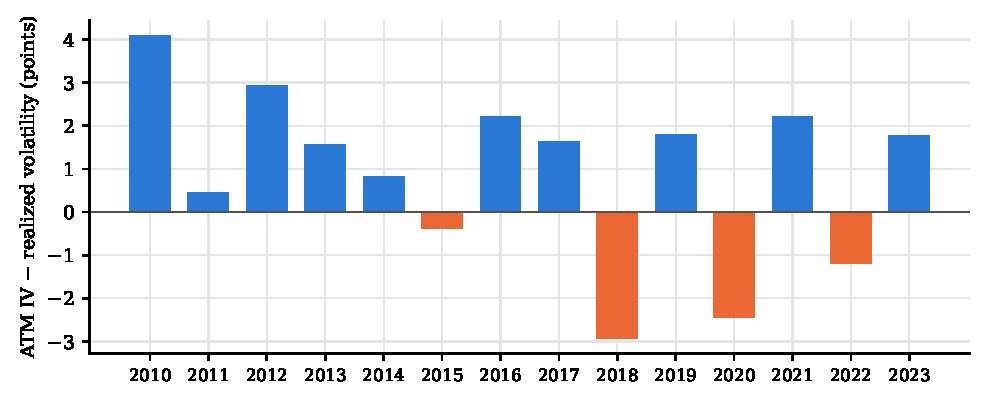
\includegraphics[width=0.85\textwidth]{anni_en.pdf}
\caption{Average 30-day at-the-money premium by year.}\label{fig:anni}
\end{figure}

\subsection{Implied volatility as a forecast}

If the option market is informationally efficient, implied volatility must be an unbiased forecast of realized volatility, up to the risk premium. The Mincer and Zarnowitz (1969) regression, $\sqrt{RV_{t,T}} = a + b\,\sigma_t + u_t$, is the standard test: under the unbiasedness hypothesis $a=0$ and $b=1$.

\begin{table}[ht]\centering\small
\caption{Mincer-Zarnowitz regressions of realized volatility on implied volatility. $a$ in volatility points; $p$-value of the joint test $a=0$, $b=1$.}\label{tab:mz}
\begin{tabular}{rrrrrrrr}\toprule
 & \multicolumn{5}{c}{ATM IV} & \multicolumn{2}{c}{Model-free} \\ \cmidrule(lr){2-6}\cmidrule(lr){7-8}
Days & $a$ & $b$ & s.e. $b$ & $R^2$ & $p$ & $b$ & $p$ \\ \midrule
7 & $-$1.35 & 1.001 & 0.084 & 0.60 & 0.000 & 0.959 & 0.000 \\
14 & $-$1.34 & 1.031 & 0.109 & 0.55 & 0.001 & 0.981 & 0.000 \\
21 & $-$0.46 & 0.980 & 0.115 & 0.47 & 0.080 & 0.928 & 0.000 \\
30 & +0.69 & 0.908 & 0.099 & 0.39 & 0.409 & 0.841 & 0.000 \\
45 & +2.14 & 0.816 & 0.071 & 0.31 & 0.035 & 0.737 & 0.000 \\
60 & +3.08 & 0.752 & 0.072 & 0.25 & 0.002 & 0.662 & 0.000 \\
\bottomrule\end{tabular}\end{table}

At 30 days the estimated slope is 0.908 (standard error 0.099) and the joint hypothesis is not rejected ($p=$ 0.409): at-the-money volatility is, in the sample, a statistically unbiased forecast. The same hypothesis is clearly rejected for the model-free measure at every horizon, as expected for a measure that embeds the premium for the tails. At 7 and 14 days the slope is close to one and the rejection of the joint hypothesis depends on the constant alone, that is, on the average premium. At the 45- and 60-day horizons the slope falls below one for the at-the-money measure as well: high implied volatility overstates subsequent realized volatility.

\begin{figure}[ht]\centering
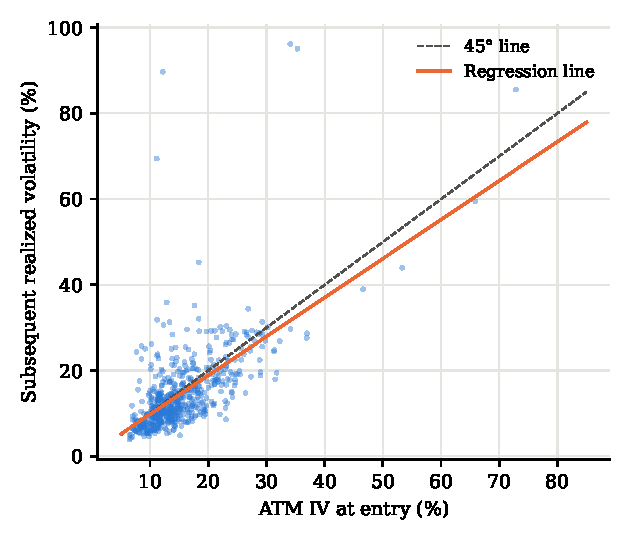
\includegraphics[width=0.46\textwidth]{mz_en.pdf}\hfill
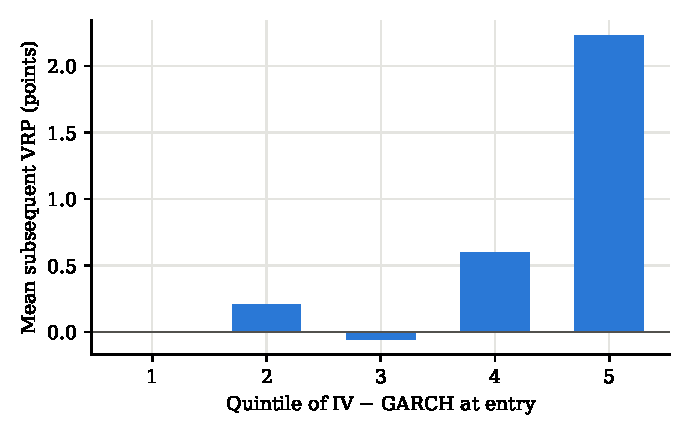
\includegraphics[width=0.50\textwidth]{gap_en.pdf}
\caption{Left: realized volatility against 30-day at-the-money implied volatility. Right: mean subsequent premium by quintile of the difference between implied volatility and the GJR-GARCH forecast at entry.}\label{fig:mz}
\end{figure}

The comparison of forecasts on the 2012--2023 sample (2,920 sessions, 30-day horizon) confirms the ranking known in the literature. The root mean squared error is 7.38 points for at-the-money volatility, 8.15 for model-free, 8.26 for GJR-GARCH and 9.22 for 21-session historical volatility. In the regression that includes the three forecasts, the coefficient of implied volatility is +0.73 ($t$ 6.50), that of GJR-GARCH +0.27 ($t$ 1.77) and that of historical volatility $-$0.09 ($t$ $-$1.01), with an $R^2$ of 0.41. The GARCH model adds marginal information of weak significance to that already contained in option prices; historical volatility adds none.

\subsection{The implied-minus-GARCH signal}

The project proposed the comparison between implied volatility and the GARCH forecast as an entry filter. Sorting sessions into quintiles of the difference $\sigma_{\mathrm{ATM}}-\sigma_{\mathrm{GARCH}}$, the mean subsequent premium is +0.00, +0.21, $-$0.05, +0.60 and +2.23 points from the first to the fifth quintile (Figure~\ref{fig:mz}). The relation is increasing and concentrated in the last quintile; the regression of the subsequent premium on the difference has a slope of 0.21 with $t$ 1.55 and an $R^2$ of 1.5\%. The signal has the expected sign but does not reach conventional significance.

\subsection{The price of insurance}

A direct measure of the premium contained in puts is the ratio of losses at expiry to premiums collected by those who sold them (Table~\ref{tab:ins}). A ratio of one corresponds to a fair price under the real-world measure. In the sample, for the 0.10-delta put the ratio is 0.44 at 30 days and 0.57 at 7 days: buyers recovered about half of the premium paid. The ratio increases toward the money (0.65 for the 0.30 delta at 30 days) and toward short maturities. This is the result of Bondarenko (2014) on a later sample. The caveat of Broadie, Chernov and Johannes (2009) applies in full: fourteen years contain a single event the size of March 2020 and none the size of October 1987.

\begin{table}[ht]\centering\small
\caption{Puts sold and held to expiry: losses at expiry relative to premiums collected (mid prices) and share of trades finishing in the money.}\label{tab:ins}
\begin{tabular}{rrrrrrr}\toprule
 & \multicolumn{4}{c}{Losses / premiums by delta} & \multicolumn{2}{c}{\% in the money} \\ \cmidrule(lr){2-5}\cmidrule(lr){6-7}
Days & 0.10 & 0.16 & 0.20 & 0.30 & 0.10 & 0.30 \\ \midrule
7 & 0.57 & 0.67 & 0.72 & 0.80 & 4.8 & 21.1 \\
14 & 0.53 & 0.64 & 0.68 & 0.74 & 4.5 & 18.8 \\
30 & 0.44 & 0.51 & 0.56 & 0.65 & 3.3 & 17.2 \\
45 & 0.44 & 0.48 & 0.51 & 0.58 & 3.0 & 15.8 \\
\bottomrule\end{tabular}\end{table}

\section{Strategies}\label{sec:strat}

\subsection{Results by family}

Table~\ref{tab:fam} reports the medians by family, held to expiry, over all combinations of delta and maturity.

\begin{table}[ht]\centering\small
\caption{Medians by family, held to expiry. Annualized Sharpe ratio of the monthly series at mid and bid-ask prices; beta and $t$-statistic of alpha against the index; spread paid as a percentage of premium traded; share of winning trades at bid-ask prices.}\label{tab:fam}
\begin{tabular}{lrrrrrrrr}\toprule
 & & \multicolumn{2}{c}{Sharpe} & & \multicolumn{2}{c}{$t$ alpha} & Spread & Wins \\ \cmidrule(lr){3-4}\cmidrule(lr){6-7}
Family & $N$ & mid & b.-a. & Beta & mid & b.-a. & \% & \% \\ \midrule
Short put & 16 & +0.89 & +0.81 & +0.57 & +1.56 & +1.38 & 3 & 92 \\
Short strangle & 16 & +0.62 & +0.52 & +0.29 & +1.17 & +0.92 & 3 & 75 \\
Put credit spread, $\Delta$ 0.05 wing & 16 & +0.84 & +0.61 & +1.89 & +1.44 & +0.47 & 6 & 92 \\
Put credit spread, 1\% of spot wing & 16 & +0.69 & $-$0.04 & +3.14 & +0.84 & $-$1.83 & 23 & 84 \\
Short ATM straddle & 4 & +0.40 & +0.17 & +0.55 & +0.50 & $-$0.11 & 2 & 58 \\
Iron condor, $\Delta$ 0.05 wing & 16 & +0.31 & $-$0.08 & +0.89 & +0.34 & $-$0.81 & 7 & 72 \\
Iron condor, 1\% of spot wing & 16 & $-$0.33 & $-$1.22 & $-$0.08 & $-$1.14 & $-$4.01 & 17 & 66 \\
Iron butterfly & 8 & +0.02 & $-$0.29 & +1.47 & $-$0.70 & $-$1.58 & 2 & 51 \\
Call credit spread, $\Delta$ 0.05 wing & 16 & $-$0.68 & $-$0.96 & $-$2.64 & $-$1.71 & $-$2.69 & 8 & 76 \\
Call credit spread, 1\% of spot wing & 16 & $-$0.79 & $-$1.21 & $-$2.97 & $-$2.01 & $-$3.96 & 13 & 74 \\
Long ATM calendar & 2 & $-$0.10 & $-$2.14 & +0.85 & $-$0.22 & $-$6.40 & 13 & 36 \\
Debit put spread & 4 & $-$0.63 & $-$0.82 & $-$26.69 & $-$0.64 & $-$1.37 & 5 & 15 \\
Long put & 8 & $-$0.84 & $-$0.90 & $-$28.96 & $-$1.35 & $-$1.54 & 3 & 8 \\
\bottomrule\end{tabular}\end{table}

The ranking is clear and follows the location of the premium. Structures that sell puts have a positive Sharpe ratio; symmetric structures (straddle, iron condor, iron butterfly) have results close to zero at mid prices and negative at bid-ask prices; structures that sell calls have negative results, because in a rising market out-of-the-money calls were exercised more often than their price implied; structures that buy options (put, debit put spread, calendar) lose. The long at-the-money calendar has a result of about zero at mid prices and strongly negative after costs, because it requires three trades in options whose spread is wide relative to the debit invested.

Wing width is decisive. With 0.05-delta wings the spread paid by a put credit spread is about 5\% of the premium traded; with wings at 1\% of spot it rises to 25\%, and the Sharpe ratio of the 0.20-delta, 30-day put credit spread goes from +0.83 to $-$0.02. Narrow structures, which are the ones accessible with limited capital, are also those on which the execution cost absorbs the whole premium.

\begin{table}[ht]\centering\footnotesize
\caption{Representative configurations. Results per SPX contract at bid-ask prices, except the Sharpe ratio at mid prices. Drawdown as a percentage of capital committed to margin; annual alpha as a percentage of the same capital.}\label{tab:sel}
\resizebox{\textwidth}{!}{%
\begin{tabular}{llrrrrrrrrr}\toprule
 & & Wins & Mean & Worst & \multicolumn{2}{c}{Sharpe} & DD & & Alpha & \\ \cmidrule(lr){6-7}
Family & Parameters & \% & \$ & \$ & mid & b.-a. & \% & Beta & \% & $t$ \\ \midrule
Short put & $\Delta$0.10, 7 d & 96 & 137 & $-$26,901 & +1.41 & +1.23 & 26 & +0.39 & +8.5 & +2.58 \\
Short put & $\Delta$0.16, 45 d & 94 & 885 & $-$83,370 & +0.99 & +0.93 & 57 & +0.31 & +9.5 & +1.75 \\
Short strangle & $\Delta$0.16, 30 d & 78 & 445 & $-$90,972 & +0.61 & +0.51 & 63 & +0.26 & +6.6 & +0.91 \\
Put credit spread & $\Delta$0.20/0.05, 30 d & 91 & 456 & $-$32,254 & +0.98 & +0.83 & 93 & +1.14 & +16.8 & +1.58 \\
Put credit spread & $\Delta$0.20, 1\%, 30 d & 85 & $-$11 & $-$7,458 & +0.75 & $-$0.02 & 235 & +2.04 & $-$24.7 & $-$1.44 \\
Put credit spread & $\Delta$0.20/0.05, 30, TP50 d & 95 & 232 & $-$32,254 & +1.02 & +0.65 & 51 & +0.69 & +6.8 & +1.08 \\
Put credit spread & $\Delta$0.20/0.05, 30, TP50/SL200 d & 87 & 101 & $-$14,312 & +1.03 & +0.37 & 44 & +0.76 & $-$2.8 & $-$0.76 \\
Short ATM straddle & ATM, 30 d & 57 & 112 & $-$99,331 & +0.31 & +0.18 & 131 & +0.36 & +1.1 & +0.11 \\
Iron condor & $\Delta$0.16/0.05, 30 d & 74 & 110 & $-$26,046 & +0.43 & +0.14 & 190 & +0.39 & +0.7 & +0.05 \\
Iron condor & $\Delta$0.16, 1\%, 30 d & 67 & $-$193 & $-$8,654 & $-$0.30 & $-$1.16 & 1673 & $-$0.79 & $-$110.3 & $-$3.92 \\
Iron butterfly & ATM/$\Delta$0.10, 30 d & 47 & $-$399 & $-$27,784 & $-$0.17 & $-$0.45 & 597 & +0.79 & $-$43.2 & $-$1.75 \\
Call credit spread & $\Delta$0.16/0.05, 30 d & 76 & $-$259 & $-$19,512 & $-$0.66 & $-$0.84 & 907 & $-$1.66 & $-$43.4 & $-$2.57 \\
Long ATM calendar & ATM, 30/60 d & 36 & $-$296 & $-$5,895 & $-$0.25 & $-$1.58 & 2138 & $-$0.09 & $-$151.7 & $-$5.07 \\
Long put & $\Delta$0.10, 30 d & 3 & $-$514 & $-$3,672 & $-$0.61 & $-$0.66 & 9552 & $-$21.04 & $-$424.6 & $-$1.02 \\
\bottomrule\end{tabular}}\end{table}

\begin{figure}[ht]\centering
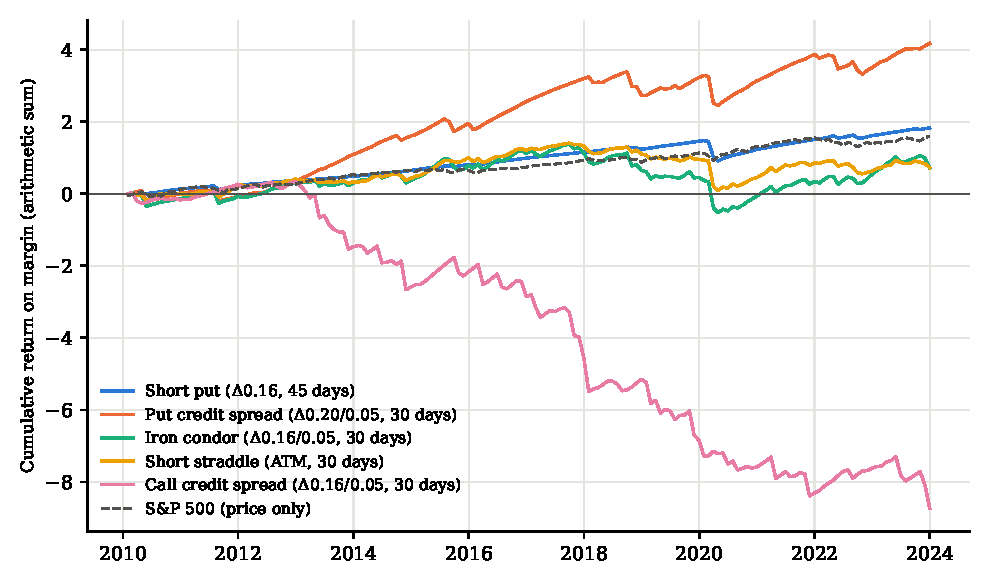
\includegraphics[width=\textwidth]{curve_en.pdf}
\caption{Cumulative return on margin (arithmetic sum of monthly returns, constant-capital ladder, bid-ask prices) for five configurations and for the index.}\label{fig:curve}
\end{figure}

\subsection{Return and risk of the best configurations}

The 0.16-delta, 45-day short put is profitable in 94\% of trades, with a mean result of 885 dollars per contract and a maximum loss of 83,370 dollars: the worst loss is more than ninety times the mean gain. The Sharpe ratio is +0.93 at bid-ask prices, above that of the index over the period (0.77, price only), but beta is 0.31 and the annual alpha, +9.5\% of margin capital, has a $t$-statistic of +1.75. The 0.20-delta put credit spread with a 0.05-delta wing at 30 days has a Sharpe ratio of +0.83, a beta of 1.14 and an alpha with $t$ +1.58; the maximum drawdown of the series equals 93\% of the capital committed to margin, which makes full deployment of capital impracticable. The 0.16-delta, 30-day iron condor has a Sharpe ratio of +0.14 and an alpha with $t$ +0.05; the short straddle, the position closest to a pure exposure to the at-the-money premium, has a Sharpe ratio of +0.18, consistent with a statistically zero at-the-money premium.

In short, positive results coincide with structures that have positive beta and for which a material part of the return is equity market exposure in a period when the index returned 11.4\% per year. This is the conclusion of Israelov and Nielsen (2015) and Jurek and Stafford (2015) applied to these strategies.

\subsection{Distribution of returns and tails}\label{sec:code}

Mean and Sharpe ratio do not describe a strategy that collects a small premium often and suffers a large loss rarely. The shape of the distribution is measured at two levels: per trade, as the return on margin at bid-ask prices with commissions, and per month, on the constant-capital ladder. The reference is a normal distribution with the same mean and variance, together with index returns over the same calendar horizon. Table~\ref{tab:code} reports skewness, excess kurtosis, the frequency of returns more than three standard deviations below the mean relative to that of the normal (0.135\%), and the 1\% expected shortfall in standard deviations relative to that of the normal (2.665). Daily entries overlap and are not independent, so the Jarque--Bera (1987) test is applied only to the monthly series.

\begin{table}[ht]\centering\footnotesize
\caption{Shape of the return distribution. Per trade: return on margin at bid-ask prices, commissions included; frequency of returns more than three standard deviations below the mean and 1\% expected shortfall in standard deviations, both relative to the normal; worst trade as a percentage of margin. Monthly: constant-capital ladder; $p$-value of the Jarque--Bera test. Last row: 30-day S\&P 500 returns from each session and monthly price returns.}\label{tab:code}
\resizebox{\textwidth}{!}{%
\begin{tabular}{llrrrrrrrr}\toprule
 & & \multicolumn{5}{c}{Per trade} & \multicolumn{3}{c}{Monthly} \\ \cmidrule(lr){3-7}\cmidrule(lr){8-10}
Family & Parameters & Skew. & Ex. kurt. & $<-3\sigma$ & ES 1\% & Worst \% & Skew. & Ex. kurt. & JB $p$ \\ \midrule
Short put & $\Delta$0.10, 7 d & $-$9.69 & 121.7 & 12.3 & 3.08 & $-$40 & $-$4.04 & 21.0 & $<$0.001 \\
Short put & $\Delta$0.16, 45 d & $-$9.47 & 108.5 & 9.8 & 3.05 & $-$125 & $-$8.67 & 91.3 & $<$0.001 \\
Short strangle & $\Delta$0.16, 30 d & $-$8.01 & 101.7 & 8.4 & 2.57 & $-$134 & $-$7.67 & 78.0 & $<$0.001 \\
Put credit spread & $\Delta$0.20/0.05, 30 d & $-$4.60 & 22.0 & 23.4 & 2.34 & $-$102 & $-$4.05 & 20.8 & $<$0.001 \\
Put credit spread & $\Delta$0.20, 1\%, 30 d & $-$2.85 & 6.6 & 53.4 & 1.35 & $-$123 & $-$2.42 & 6.1 & $<$0.001 \\
Put credit spread & $\Delta$0.20/0.05, 30, TP50 d & $-$6.11 & 39.0 & 18.4 & 2.84 & $-$102 & $-$4.24 & 21.4 & $<$0.001 \\
Put credit spread & $\Delta$0.20/0.05, 30, TP50/SL200 d & $-$2.52 & 5.5 & 18.4 & 1.62 & $-$44 & $-$1.60 & 2.7 & $<$0.001 \\
Short ATM straddle & ATM, 30 d & $-$2.92 & 23.9 & 8.3 & 2.03 & $-$148 & $-$4.20 & 33.1 & $<$0.001 \\
Iron condor & $\Delta$0.16/0.05, 30 d & $-$2.82 & 9.7 & 16.7 & 2.00 & $-$103 & $-$2.57 & 11.0 & $<$0.001 \\
Iron condor & $\Delta$0.16, 1\%, 30 d & $-$1.13 & $-$0.4 & 0.2 & 0.90 & $-$186 & $-$1.11 & 0.5 & $<$0.001 \\
Iron butterfly & ATM/$\Delta$0.10, 30 d & $-$0.41 & $-$0.1 & 0.0 & 0.97 & $-$107 & $-$0.68 & 0.8 & $<$0.001 \\
Call credit spread & $\Delta$0.16/0.05, 30 d & $-$1.99 & 2.6 & 1.9 & 1.12 & $-$110 & $-$1.89 & 3.0 & $<$0.001 \\
Long ATM calendar & ATM, 30/60 d & 0.49 & $-$0.1 & 0.0 & 0.81 & $-$189 & $-$0.22 & 0.2 & 0.473 \\
Long put & $\Delta$0.10, 30 d & 16.40 & 312.1 & 0.0 & 0.06 & $-$198 & 11.63 & 141.2 & $<$0.001 \\
\midrule
S\&P 500 & 30 d & $-$1.22 & 6.9 & 6.2 & 1.64 & $-$34 & $-$0.33 & 0.4 & 0.118 \\
\bottomrule\end{tabular}}\end{table}

Structures that sell volatility without protection have left tails far longer than those of the normal and of the index. For the 0.16-delta, 45-day short put, per-trade skewness is $-$9.5 and excess kurtosis 108, against $-$1.1 and 4.8 for index returns over 45 days; losses beyond three standard deviations are 9.8 times as frequent as under the normal and the 1\% expected shortfall is 3.0 times the normal one (Figures~\ref{fig:code} and~\ref{fig:qq}). The shape persists in the monthly series of the ladder (skewness $-$8.7, excess kurtosis 91), whereas monthly index returns are close to normal over the period (skewness $-$0.33, excess kurtosis 0.40, Jarque--Bera $p$ = 0.12). Across all 434 configurations, 96\% have negative per-trade skewness and the Jarque--Bera test rejects normality of the monthly series at the 1\% level in 92\%.

The tail of the losses is not heavier than that of the index in the asymptotic sense. Beyond the strike the loss of a position held to expiry is linear in the final price, so it inherits the tail index of the underlying: the Hill (1975) estimator on 30-day index returns, with 2.5\% of the observations in the tail, gives 2.9 (between 2.3 and 2.9 with 1 to 5\%), in line with the value close to three documented for equity indices (Gopikrishnan et al., 1999; Cont, 2001). What changes is the body of the distribution: almost all outcomes are concentrated on the premium collected, the standard deviation is small, and the rare losses lie many standard deviations away. With a tail index below four the population kurtosis is not finite (Mandelbrot, 1963), so the sample values describe 2010--2023 and depend on a few episodes; the informative part is the comparison across structures and with the index. On strategy returns the Hill estimator depends on the threshold, because the body is compressed on the premium and overlapping trades replicate the same episode, and it is not reported.

\begin{figure}[ht]\centering
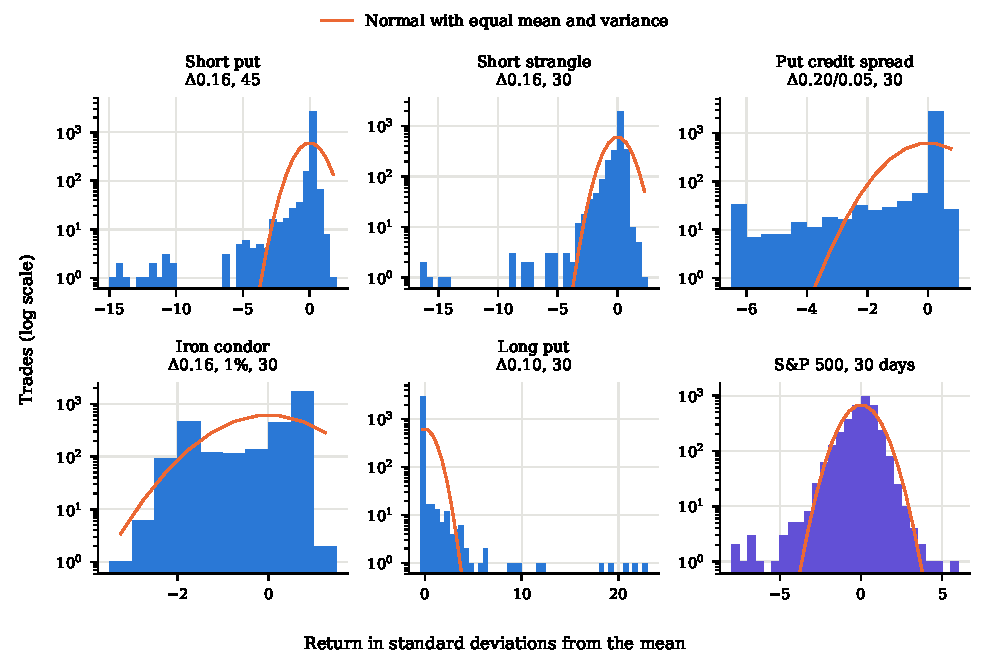
\includegraphics[width=\textwidth]{code_en.pdf}
\caption{Per-trade returns in standard deviations from the mean, bid-ask prices; number of trades on a logarithmic scale. The curve is the number expected under a normal distribution with the same mean and variance. Last panel: 30-day S\&P 500 returns from each session.}\label{fig:code}
\end{figure}

Defined-risk structures truncate the tail at the width of the spread, but truncation alone does not make the distribution normal. With 0.05-delta wings excess kurtosis remains high (22.0 for the 0.20-delta put credit spread, with losses beyond three standard deviations 23.4 times as frequent as under the normal). With wings at 1\% of spot the maximum loss becomes frequent rather than rare: 17.8\% of the trades of the 0.16-delta iron condor lose more than 90\% of margin, against 6.2\% under the normal, and excess kurtosis falls to $-$0.39. The risk is no longer a distant tail but a large probability mass at the maximum loss, which kurtosis does not capture. Exiting at a loss of 200\% of the premium brings the excess kurtosis of the put credit spread from 22.0 to 5.5; the cost of the rule is discussed in the next subsection. Structures that buy volatility have the opposite shape: positive skewness and a long right tail (0.10-delta long put: skewness 16.4), while the long 30/60-day at-the-money calendar is close to normal (Jarque--Bera $p$ = 0.47 on the monthly series).

\begin{figure}[ht]\centering
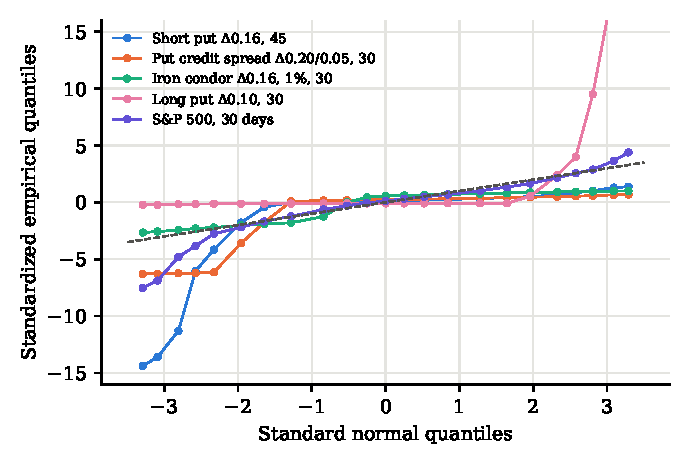
\includegraphics[width=0.7\textwidth]{qq_en.pdf}
\caption{Quantile--quantile plot of standardized per-trade returns against the standard normal; the dashed diagonal corresponds to the normal.}\label{fig:qq}
\end{figure}

Two consequences follow. Rankings based on mean and standard deviation, the Sharpe ratio included, overstate the quality of short-volatility structures: selling out-of-the-money options is the standard example of how a negatively skewed return can raise the Sharpe ratio without adding value (Goetzmann et al., 2007). The deflated Sharpe ratio of Section~\ref{sec:rob} corrects for the skewness and kurtosis of the monthly series. In the project's selection procedure, a criterion that divides expected value by a power of the standard deviation inherits the same limitation: tail risk should be measured directly, through the expected shortfall or the probability of the maximum loss under the GJR-GARCH density, and kept separate from the expected-value filter.

\subsection{Exit rules}

The median Sharpe ratio of credit structures is +0.41, +0.44 and +0.43 at mid prices for hold-to-expiry, 50\% profit-taking, and profit-taking with a 200\% loss limit respectively; at bid-ask prices it becomes $-$0.05, $-$0.44 and $-$0.73. At mid prices exit rules do not change expected return, as must be the case for a rule that contains no information; at bid-ask prices they worsen it, because every early exit pays a second spread, whereas cash settlement at expiry pays none. The rules reduce maximum drawdown, but at a certain cost.

\subsection{Entry filters}

Table~\ref{tab:filt} compares, from 2012, the median Sharpe ratio without filters with the one obtained by opening positions only when implied volatility exceeds the GARCH forecast, only when it is below it, and in the extreme terciles of the level of implied volatility. The filter $\sigma_{\mathrm{ATM}}>\sigma_{\mathrm{GARCH}}$ improves the Sharpe ratio in 86\% of credit configurations, and the median moves from $-$0.26 to $-$0.05. The improvement is systematic in sign but does not turn losing families into winning ones. For the 0.16-delta, 45-day short put the Sharpe ratio goes from +0.90 to +1.62; for the 0.16-delta, 30-day iron condor from +0.18 to +0.70. The result must be read together with that of Section~\ref{sec:vrp}: the signal has the correct sign, but its statistical significance on the premium is weak and the filter was evaluated on the same sample on which it was conceived.

\begin{table}[ht]\centering\small
\caption{Median Sharpe ratio by family and entry filter, bid-ask prices, 2012--2023. Months without trades count as zero return.}\label{tab:filt}
\begin{tabular}{lrrrrrr}\toprule
Family & $N$ & None & IV $>$ GARCH & IV $\le$ GARCH & High IV & Low IV \\ \midrule
Short put & 48 & +0.88 & +0.92 & +0.56 & +0.83 & +0.28 \\
Short strangle & 48 & +0.43 & +0.70 & +0.15 & +0.37 & +0.21 \\
Put credit spread & 96 & +0.13 & +0.24 & $-$0.04 & +0.24 & $-$0.04 \\
Short ATM straddle & 12 & +0.20 & +0.41 & $-$0.00 & +0.20 & +0.04 \\
Iron condor & 96 & $-$0.85 & $-$0.40 & $-$0.83 & $-$0.55 & $-$0.30 \\
Iron butterfly & 24 & $-$0.25 & $-$0.06 & $-$0.32 & $-$0.14 & $-$0.10 \\
Call credit spread & 96 & $-$1.27 & $-$0.83 & $-$1.02 & $-$1.00 & $-$0.55 \\
\bottomrule\end{tabular}\end{table}

\subsection{Operational filter on realized volatility}\label{sec:fvol}

A common prudential rule is to suspend new trades when realized volatility is excessive and to resume when it subsides, with the aim of avoiding extreme events. The rule was tested on all credit configurations: entries are suspended when 21-session historical volatility (HV21) exceeds a threshold and resume when it falls back below; positions already open follow their own management. The thresholds are 20\%, 25\% and 30\% annualized and the 90th percentile computed only on data already observed (Table~\ref{tab:fvol}).

\begin{table}[ht]\centering\small
\caption{Suspension of entries as a function of realized volatility: medians across credit configurations, bid-ask prices, March 2011--December 2023. Drawdown and worst month as a percentage of capital committed to margin.}\label{tab:fvol}
\begin{tabular}{lrrrrrr}\toprule
 & Trades & Median & Sharpe & Median & Drawdown & Worst \\
Filter & executed \% & Sharpe & better \% & drawdown \% & smaller \% & month \% \\ \midrule
No filter & 100 & $-$0.30 & -- & 393 & -- & $-$69 \\
HV21 $\le$ 20\% & 82 & $-$0.37 & 49 & 324 & 85 & $-$64 \\
HV21 $\le$ 25\% & 91 & $-$0.34 & 45 & 343 & 82 & $-$65 \\
HV21 $\le$ 30\% & 97 & $-$0.30 & 46 & 370 & 73 & $-$67 \\
HV21 $\le$ 90th percentile & 90 & $-$0.35 & 42 & 356 & 80 & $-$65 \\
HV10 $\le$ 25\% & 91 & $-$0.36 & 38 & 377 & 69 & $-$65 \\
Only HV21 $>$ 25\% & 9 & +0.07 & 76 & 55 & 100 & $-$31 \\
\bottomrule\end{tabular}\end{table}

There are three results. First, the filter does not improve risk-adjusted return. With the 25\% threshold the median Sharpe ratio moves from $-$0.30 to $-$0.34 and improves in only 45\% of configurations; for the 0.16-delta, 45-day short put it falls from +0.89 to +0.64, for the 0.16-delta, 30-day iron condor from +0.17 to +0.08. Second, drawdown falls in 82\% of configurations, but by an amount close to the reduction in the number of trades (91\% of those without the filter), and the worst month does not change: for the short put it remains 43.9\% of margin capital with and without the filter. The positions that suffered the largest losses, in February 2020, had been opened with low realized volatility: the filter suspends entries after the event, not before. Third, trades opened with HV21 above 25\% have an above-average mean return per trade (for the short put 5.2\% of margin against 1.8\%), so the filter gives up precisely the best-paid trades.

\begin{table}[ht]\centering\small
\caption{Subsequent 30-day premium by level of 21-session historical volatility at entry. Values in volatility points.}\label{tab:hv}
\begin{tabular}{lrrrrrrrrr}\toprule
HV21 (\%) & Sessions & ATM IV & Real. & ATM $-$ real. & $t$ & MF $-$ real. & \% $>0$ & 5th pct. & Min. \\ \midrule
$\le$ 10 & 998 & 10.79 & 11.01 & $-$0.22 & $-$0.44 & +2.36 & 61 & $-$10.2 & $-$21 \\
10--15 & 1,041 & 13.77 & 12.72 & +1.05 & 1.47 & +3.56 & 77 & $-$5.8 & $-$77 \\
15--20 & 529 & 17.26 & 15.71 & +1.55 & 1.85 & +4.35 & 72 & $-$9.2 & $-$72 \\
20--25 & 269 & 20.91 & 19.69 & +1.21 & 1.05 & +4.47 & 67 & $-$9.3 & $-$70 \\
25--30 & 176 & 24.09 & 22.50 & +1.58 & 1.43 & +4.75 & 66 & $-$6.9 & $-$68 \\
$>$ 30 & 115 & 33.14 & 33.45 & $-$0.31 & $-$0.10 & +3.63 & 68 & $-$42.0 & $-$68 \\
\bottomrule\end{tabular}\end{table}

Table~\ref{tab:hv} shows why. The subsequent at-the-money premium does not decline when realized volatility is high: it is close to zero in the two extreme classes ($-$0.22 points with HV21 below 10\%, $-$0.31 points above 30\%) and positive in the intermediate ones. Extreme losses originate in calm phases: the minimum of the premium belongs to the 10--15\% class. Above 30\% dispersion is very wide and the sample small, and none of the class means is statistically different from zero.

The filter is also redundant given how the strategies are built. Strikes are chosen by delta on market implied volatility, so the structure widens by itself when volatility rises: the distance from the forward of the 0.16-delta, 30-day put averages 3.8\% in the low implied volatility tercile (mean IV 10.0\%), 5.0\% in the middle tercile and 7.5\% in the high tercile (mean IV 22.2\%), with a correlation of 0.98 between distance and implied volatility. In the project's selection procedure the GJR-GARCH density plays the same role on expected value and probabilities: a higher forecast volatility widens the distribution and moves the selection toward wider structures or rules it out. Volatility is therefore already embedded twice, in strike placement and in the expected-value filter.

The operational conclusion is that a suspension based on realized volatility is not necessary and does not protect against extreme events, which by definition arrive from calm conditions. It is equivalent to a reduction in exposure, obtainable more directly through the share of capital committed to margin; protection against the tails rests on the defined risk of the structures and on sizing.

\section{Robustness and multiple testing}\label{sec:rob}

\subsection{Execution cost}

Across 434 configurations the median Sharpe ratio is +0.39 at mid prices and $-$0.40 at bid-ask prices; the share of configurations with a positive Sharpe ratio falls from 64\% to 38\% (Figure~\ref{fig:sharpe}). The actual execution price lies between the two extremes: closing quotes overstate the spread typical of the middle of the session, but a mid-price order on a multi-leg structure has no guarantee of execution. The site lets the share of spread paid be set and recomputes every statistic.

\begin{figure}[ht]\centering
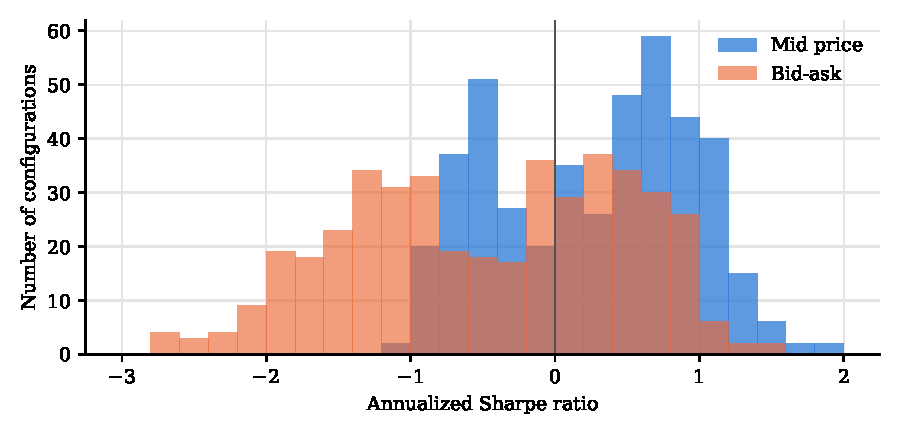
\includegraphics[width=0.54\textwidth]{sharpe_en.pdf}\hfill
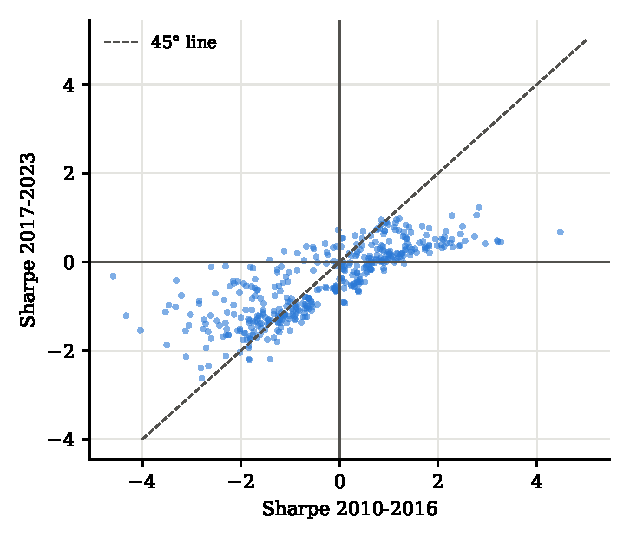
\includegraphics[width=0.42\textwidth]{meta_en.pdf}
\caption{Left: distribution of the Sharpe ratio across the 434 configurations, at mid and bid-ask prices. Right: Sharpe ratio in 2010--2016 and in 2017--2023 for credit configurations.}\label{fig:sharpe}
\end{figure}

\subsection{Alpha against the index}

The share of configurations with positive alpha and a $t$-statistic above 2 is 16.4\% at mid prices and 2.5\% at bid-ask prices. Under the null hypothesis of zero alpha for all configurations, the share expected by chance alone is about 2.5\%. By contrast, 49.8\% of configurations have a significantly negative alpha at bid-ask prices. At prices that can actually be traded, the evidence of return in excess of equity exposure cannot be distinguished from what would be expected in the absence of any capturable premium.

\subsection{Ex-post selection}

Among 434 configurations the best has a Sharpe ratio of 1.58. The expected maximum under the null, computed following Bailey and López de Prado (2014) from the dispersion of observed Sharpe ratios, is 2.85; the deflated Sharpe ratio of the best configuration is 0.012. The measure is conservative, because the dispersion includes true differences across families and the trials are not independent; it nevertheless indicates that the observed maximum is not, by itself, evidence of a positive expected return.

A more direct check is the sample split. The rank correlation between the Sharpe ratio in 2010--2016 and in 2017--2023 is 0.84: the ordering across families is stable. The level is not: the twenty best configurations in the first period have a mean Sharpe ratio of 2.67 in the first and 0.60 in the second, while the median of all credit configurations in the second period is $-$0.44. A parameter chosen on the past keeps its relative position and loses about three quarters of the result.

\section{Checks on the pre-existing code}\label{sec:codice}

The reconstruction required reading the code in the group's repository. The points that change numerical results are reported below, with the file concerned.

\begin{enumerate}
\item \texttt{vrp\_analysis.py} and \texttt{utils\_vrp\_analysis.py}. ``Future'' realized volatility is computed as \texttt{rets.shift(-1).rolling(window=dte).std()}. The rolling window looks backward: the expression uses returns from $t-\mathrm{dte}+2$ to $t+1$, that is, past volatility shifted by one session. The ``IV minus future RV'' charts therefore compare implied volatility with past realized volatility. The correct form is \texttt{rets.rolling(n).std().shift(-n)}, with $n$ in sessions.
\item In the same files and in \texttt{utils\_forecast\_price\_distribution.py} the time to expiry in calendar days is used as a number of sessions. For an option with 20 calendar days the forecast cumulates 20 daily variances instead of about 14, and the standard deviation of the forecast distribution is overstated by a factor $\sqrt{20/14}\approx 1.20$. The effect is a systematic understatement of the expected value of short structures.
\item In \texttt{utils\_forecast\_price\_distribution.py} prices are downloaded up to the expiry date and estimation uses data up to $h$ sessions before the last one: for $h=20$ the window ends about six sessions before the entry date, and the starting price of the distribution is not the entry price. There is no look-ahead, but forecast and trade are not aligned.
\item In \texttt{generate\_signal\_garch\_vs\_iv.py} the branch that should generate the long-volatility signal (\texttt{spread <= -0.01}) is preceded by the branch \texttt{spread < 0.00} and is never executed.
\item In \texttt{utils\_criteria.py} the \texttt{payoff} argument is overwritten at the top of the function by a test vector; the criteria returned do not depend on the strategy passed.
\item The \texttt{.gitattributes} file of the main development branch contains an invalid line, the residue of a merge conflict, and the repository's Git LFS quota is exhausted: \texttt{.pkl} and \texttt{.csv} files can no longer be downloaded. The analyses in this document start from the original compressed archives, which are in the repository without LFS.
\end{enumerate}

The group's historical result on the 10-day iron condor (annualized return of 1.85\%, 57.3\% winning trades, maximum drawdown above half of capital) is consistent, in sign and order of magnitude, with the results obtained here for the same family.

\section{Limitations}\label{sec:limiti}

\emph{Data.} Quotes are end-of-day; the spread at the close is wider than the typical intraday spread, and closing prices of options and index may not be synchronous. Monthly expiries with settlement at the open are valued at the close of the expiry day. The sample covers fourteen years of a predominantly rising market.

\emph{Margin.} The margin of naked positions is approximated by 20\% of notional; actual margin depends on the broker and the regime, and under stress it rises just when the position is losing. The series do not include the return on cash collateral.

\emph{Design.} Every session opens a unit position, with no dynamic sizing. The monthly series assigns the result to the closing month and does not mark open positions to market: intra-month drawdown is understated. Alpha is estimated against the index alone.

\emph{Selection.} The families and parameters are those the project has explored over the years on the same archive: no part of the sample is truly out of sample. The only uncontaminated check is recording signals before the outcome is known.

\section{Conclusions}\label{sec:concl}

On SPX chains from 2010 to 2023 the volatility risk premium exists in the form described by the literature: model-free implied variance exceeds realized variance by a large and significant amount, out-of-the-money puts returned about half of the premium to buyers, and the distribution of the realized premium is dominated by a few extreme events. By contrast, there is no significant premium in the sample on at-the-money volatility beyond two weeks: at that level implied volatility is an unbiased forecast of realized volatility and outperforms both the GARCH model and historical volatility. The market appears informationally efficient at the center of the surface and rewards tail risk in the wings.

For the project's strategies there are three consequences. First, symmetric defined-risk structures, the iron condor in particular, sell both the part of the surface that contains the premium (puts) and the part that does not (calls), and pay the spread on four legs; the net result is zero or negative. Second, structures that sell puts keep a positive result after costs, but a material part is equity market exposure and the residual alpha is not statistically distinguishable from zero in the great majority of configurations. Third, exit rules and filters change the distribution of results but do not create expected return; suspending entries when realized volatility is high reduces exposure without avoiding extreme events, because delta-selected strikes already widen with implied volatility; the filter based on the comparison with GARCH has the correct sign and deserves a forward test.

The distribution of returns qualifies every Sharpe ratio in this paper. Structures that sell volatility have per-trade skewness and kurtosis far beyond those of the index, and the monthly series is not normal in 92\% of configurations: tail risk has to be measured directly, not inferred from the standard deviation.

The working hypothesis that the premium exists but that the attempt to capture it systematically tends, over the long run and net of costs, to a zero result is not rejected by the data.

\appendix
\section{Payoff at expiry of the structures}\label{app:payoff}

With $S_T$ the index value at expiry and premiums in index points, payoffs per unit are as follows. Short put with strike $B$ and premium $P_B$: $P_B - \max(B-S_T,0)$. Put credit spread with strikes $A<B$: credit $c=P_B-P_A$, payoff $c - \max(B-S_T,0) + \max(A-S_T,0)$, maximum loss $(B-A)-c$, break-even $B-c$. Iron condor with strikes $A<B<C<D$: credit $c=(P_B+C_C)-(P_A+C_D)$, payoff
\[
c - \max(B-S_T,0) + \max(A-S_T,0) - \max(S_T-C,0) + \max(S_T-D,0),
\]
maximum loss $\max(B-A,\,D-C)-c$, break-evens $B-c$ and $C+c$. The iron butterfly is the case $B=C$. For the put calendar with strike $K$, sold at expiry $T_1$ and bought at expiry $T_2>T_1$, the result at the first expiry is $P(K,T_2;T_1) - \max(K-S_{T_1},0) - d$, with $d$ the initial debit and $P(K,T_2;T_1)$ the market value of the surviving leg at $T_1$. All dollar values are obtained by multiplying by 100.

\begin{thebibliography}{99}\small
\bibitem{} Bailey, D. H. and López de Prado, M. (2014). The deflated Sharpe ratio: correcting for selection bias, backtest overfitting, and non-normality. \emph{Journal of Portfolio Management}, 40(5), 94--107.
\bibitem{} Bakshi, G. and Kapadia, N. (2003). Delta-hedged gains and the negative market volatility risk premium. \emph{Review of Financial Studies}, 16(2), 527--566.
\bibitem{} Bates, D. S. (2000). Post-'87 crash fears in the S\&P 500 futures option market. \emph{Journal of Econometrics}, 94(1--2), 181--238.
\bibitem{} Beckmeyer, H., Branger, N. and Gayda, L. (2023). Retail traders love 0DTE options... but should they? Working paper, SSRN.
\bibitem{} Black, F. (1976). The pricing of commodity contracts. \emph{Journal of Financial Economics}, 3(1--2), 167--179.
\bibitem{} Black, F. and Scholes, M. (1973). The pricing of options and corporate liabilities. \emph{Journal of Political Economy}, 81(3), 637--654.
\bibitem{} Bollen, N. P. B. and Whaley, R. E. (2004). Does net buying pressure affect the shape of implied volatility functions? \emph{Journal of Finance}, 59(2), 711--753.
\bibitem{} Bollerslev, T. (1986). Generalized autoregressive conditional heteroskedasticity. \emph{Journal of Econometrics}, 31(3), 307--327.
\bibitem{} Bollerslev, T., Tauchen, G. and Zhou, H. (2009). Expected stock returns and variance risk premia. \emph{Review of Financial Studies}, 22(11), 4463--4492.
\bibitem{} Bollerslev, T. and Todorov, V. (2011). Tails, fears, and risk premia. \emph{Journal of Finance}, 66(6), 2165--2211.
\bibitem{} Bondarenko, O. (2014). Why are put options so expensive? \emph{Quarterly Journal of Finance}, 4(3), 1450015.
\bibitem{} Britten-Jones, M. and Neuberger, A. (2000). Option prices, implied price processes, and stochastic volatility. \emph{Journal of Finance}, 55(2), 839--866.
\bibitem{} Broadie, M., Chernov, M. and Johannes, M. (2009). Understanding index option returns. \emph{Review of Financial Studies}, 22(11), 4493--4529.
\bibitem{} Canina, L. and Figlewski, S. (1993). The informational content of implied volatility. \emph{Review of Financial Studies}, 6(3), 659--681.
\bibitem{} Carr, P. and Wu, L. (2009). Variance risk premiums. \emph{Review of Financial Studies}, 22(3), 1311--1341.
\bibitem{} Christensen, B. J. and Prabhala, N. R. (1998). The relation between implied and realized volatility. \emph{Journal of Financial Economics}, 50(2), 125--150.
\bibitem{} Constantinides, G. M., Jackwerth, J. C. and Savov, A. (2013). The puzzle of index option returns. \emph{Review of Asset Pricing Studies}, 3(2), 229--257.
\bibitem{} Cont, R. (2001). Empirical properties of asset returns: stylized facts and statistical issues. \emph{Quantitative Finance}, 1(2), 223--236.
\bibitem{} Coval, J. D. and Shumway, T. (2001). Expected option returns. \emph{Journal of Finance}, 56(3), 983--1009.
\bibitem{} Dew-Becker, I. and Giglio, S. (2023). Risk preferences implied by synthetic options. NBER Working Paper 31833.
\bibitem{} Dew-Becker, I. and Giglio, S. (2025). The decline of the variance risk premium: evidence from traded and synthetic options. Federal Reserve Bank of Chicago, Working Paper 2025-17.
\bibitem{} Dew-Becker, I., Giglio, S., Le, A. and Rodriguez, M. (2017). The price of variance risk. \emph{Journal of Financial Economics}, 123(2), 225--250.
\bibitem{} Engle, R. F. (1982). Autoregressive conditional heteroscedasticity with estimates of the variance of United Kingdom inflation. \emph{Econometrica}, 50(4), 987--1007.
\bibitem{} Fama, E. F. (1970). Efficient capital markets: a review of theory and empirical work. \emph{Journal of Finance}, 25(2), 383--417.
\bibitem{} Gârleanu, N., Pedersen, L. H. and Poteshman, A. M. (2009). Demand-based option pricing. \emph{Review of Financial Studies}, 22(10), 4259--4299.
\bibitem{} Glosten, L. R., Jagannathan, R. and Runkle, D. E. (1993). On the relation between the expected value and the volatility of the nominal excess return on stocks. \emph{Journal of Finance}, 48(5), 1779--1801.
\bibitem{} Goetzmann, W., Ingersoll, J., Spiegel, M. and Welch, I. (2007). Portfolio performance manipulation and manipulation-proof performance measures. \emph{Review of Financial Studies}, 20(5), 1503--1546.
\bibitem{} Gopikrishnan, P., Plerou, V., Amaral, L. A. N., Meyer, M. and Stanley, H. E. (1999). Scaling of the distribution of fluctuations of financial market indices. \emph{Physical Review E}, 60(5), 5305--5316.
\bibitem{} Hill, B. M. (1975). A simple general approach to inference about the tail of a distribution. \emph{Annals of Statistics}, 3(5), 1163--1174.
\bibitem{} Ilmanen, A. (2012). Do financial markets reward buying or selling insurance and lottery tickets? \emph{Financial Analysts Journal}, 68(5), 26--36.
\bibitem{} Israelov, R. and Nielsen, L. N. (2015). Covered calls uncovered. \emph{Financial Analysts Journal}, 71(6), 44--57.
\bibitem{} Jackwerth, J. C. (2000). Recovering risk aversion from option prices and realized returns. \emph{Review of Financial Studies}, 13(2), 433--451.
\bibitem{} Jarque, C. M. and Bera, A. K. (1987). A test for normality of observations and regression residuals. \emph{International Statistical Review}, 55(2), 163--172.
\bibitem{} Jiang, G. J. and Tian, Y. S. (2005). The model-free implied volatility and its information content. \emph{Review of Financial Studies}, 18(4), 1305--1342.
\bibitem{} Jurek, J. W. and Stafford, E. (2015). The cost of capital for alternative investments. \emph{Journal of Finance}, 70(5), 2185--2226.
\bibitem{} Mandelbrot, B. (1963). The variation of certain speculative prices. \emph{Journal of Business}, 36(4), 394--419.
\bibitem{} Mincer, J. and Zarnowitz, V. (1969). The evaluation of economic forecasts. In J. Mincer (ed.), \emph{Economic Forecasts and Expectations}. NBER.
\bibitem{} Newey, W. K. and West, K. D. (1987). A simple, positive semi-definite, heteroskedasticity and autocorrelation consistent covariance matrix. \emph{Econometrica}, 55(3), 703--708.
\bibitem{} Poon, S.-H. and Granger, C. W. J. (2003). Forecasting volatility in financial markets: a review. \emph{Journal of Economic Literature}, 41(2), 478--539.
\bibitem{} Santa-Clara, P. and Saretto, A. (2009). Option strategies: good deals and margin calls. \emph{Journal of Financial Markets}, 12(3), 391--417.
\bibitem{} Todorov, V. (2010). Variance risk-premium dynamics: the role of jumps. \emph{Review of Financial Studies}, 23(1), 345--383.
\end{thebibliography}
\end{document}
